\documentclass{article}
\usepackage{graphicx}
\usepackage{caption}
\usepackage{float}
\usepackage[margin=1.5in]{geometry}
\author{Arvind Ramachandran}
\title{Modeling and Forecasting Trend, Seasonality, and Cycles}
\date{May 31 2019}

\begin{document}
\maketitle
\section{Introduction}

In this project, we will model the non-adjusted monthly unemployment rates in California and New York from January 1976 to April 2019. The time series data was downloaded from the website of the Federal Reserve Bank of St. Louis. \\

\noindent We will use ARIMA models on the individual time series to product a model and forecast unemployment rates into the future in both California and New York. We will then use a vector auto-regressive model to create a joint model wherein the unemployment rates for the states are dependent on past unemployment in the same state as well as in the other state.
\newpage
\section{Results}
(a) The time series plots for unemployment in California and New York are shown below, along with the ACF and PACF plots for both states. The partial autocorrelation plots for both states spike at values 1 and 12, suggesting that a seasonal (one-year) and lag-1 autoregressive component. We will thus fit both time series to an seasonal ARIMA (1,0,0), (0,0,12) model.
\begin{figure}[H]

	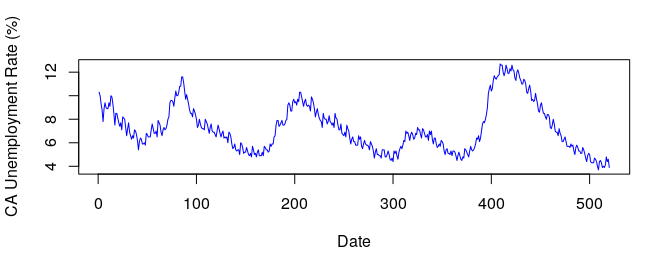
\includegraphics[width=\linewidth]{ca_ts}
		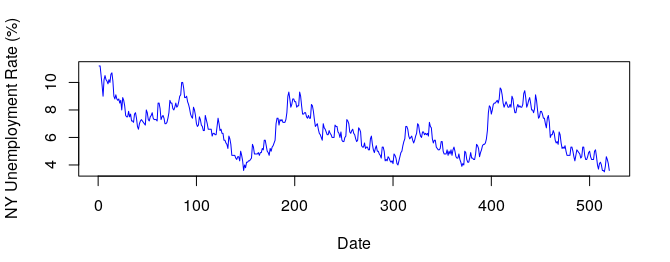
\includegraphics[width=\linewidth]{ny_ts}
			\caption{California and New York Unemployment Rates} 
\end{figure}
\begin{figure}[H]
	
	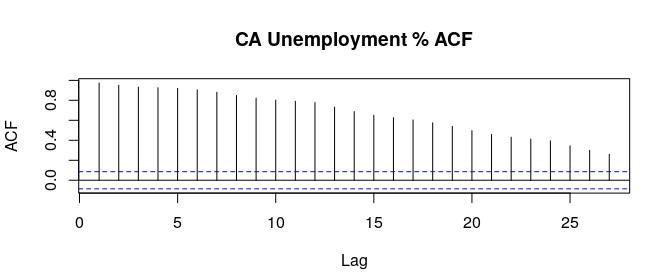
\includegraphics[width=\linewidth]{ca_acf}
	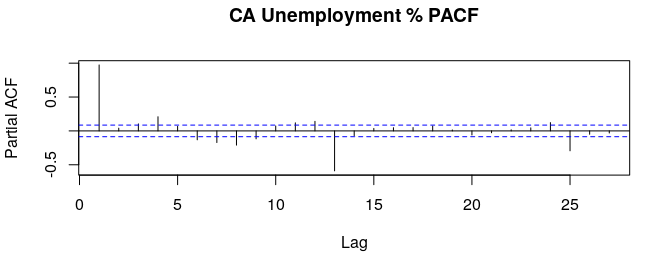
\includegraphics[width=\linewidth]{ca_pacf}
	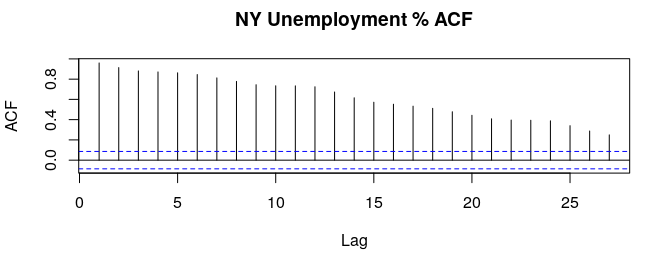
\includegraphics[width=\linewidth]{ny_acf}
	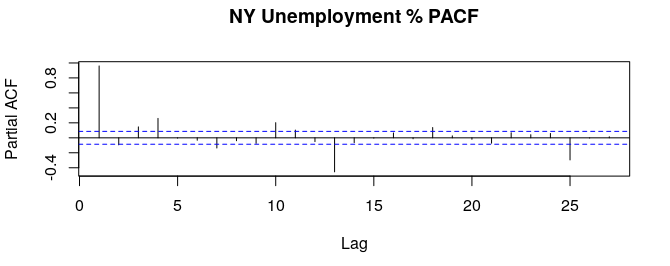
\includegraphics[width=\linewidth]{ny_pacf}
	\caption{ACFs and PACFs} 
\end{figure}
 \noindent(b \& c) The fit from the ARIMA (1,0,0), (0,0,12) model is shown below, along with the residuals. We notice that the model does a very good job fitting the time series, although it has not accounted for all the seasonality. I compared these with the best-fit ARIMA models, but the auto.arima models do not produce a much better fit.
 \begin{figure}[H]
 	
 	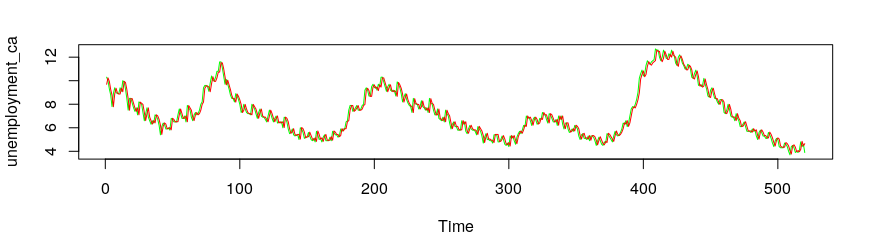
\includegraphics[width=330pt]{ca_arima_fit}
 	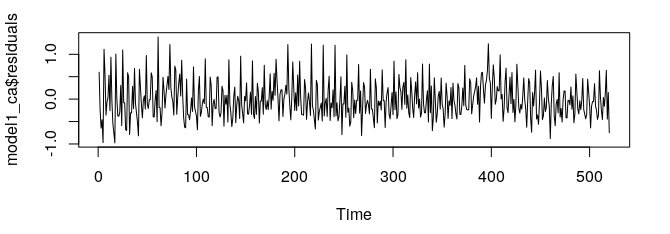
\includegraphics[width=330pt]{CA_residuals}
 	\caption{California ARIMA Model -  In the first plot, the green line is the original time series and the red line is the model fit. The second plot shows the model residuals.} 
 \end{figure}
 \begin{figure}[H]
	
	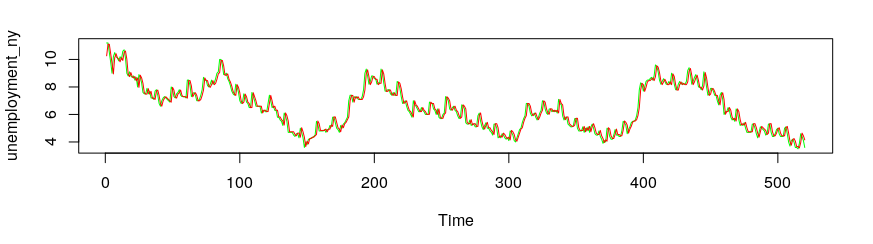
\includegraphics[width=330pt]{ny_arima_fit}
	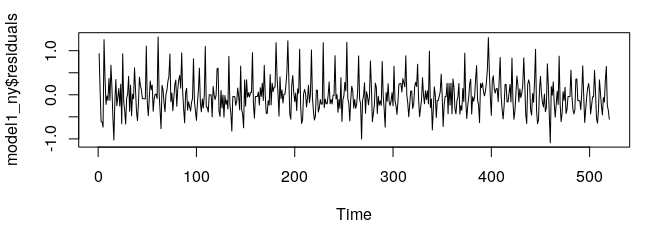
\includegraphics[width=330pt]{ny_residuals}
	\caption{New York ARIMA Model -  In the first plot, the green line is the original time series and the red line is the model fit. The second plot shows the model residuals.} 
\end{figure}

\noindent (e) The ACF and PACF plots of the residuals show that there is some remaining autoregressive component, which indicates (as we said above) that the model has not fully fit the seasonality of the unemployment time series. 
 \begin{figure}[H]
	
	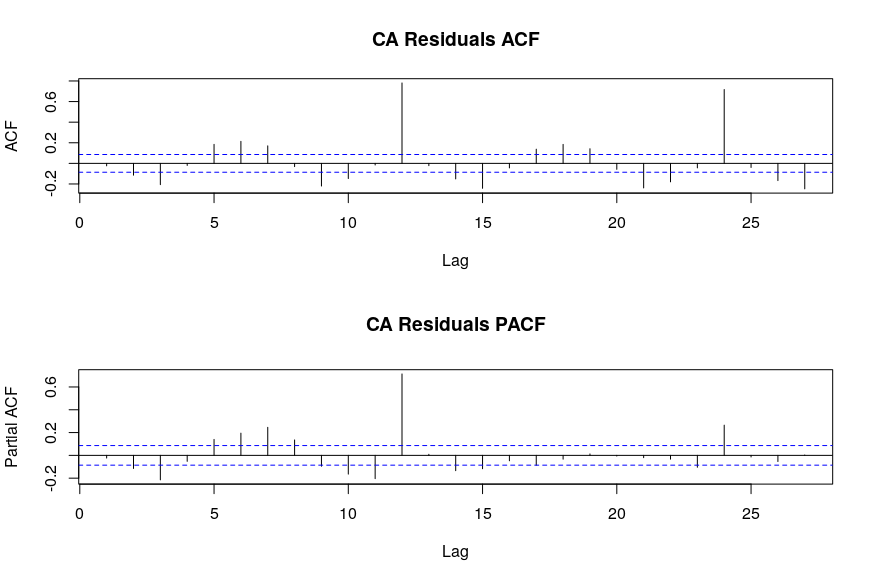
\includegraphics[width=380pt]{ca_residuals_acf}
	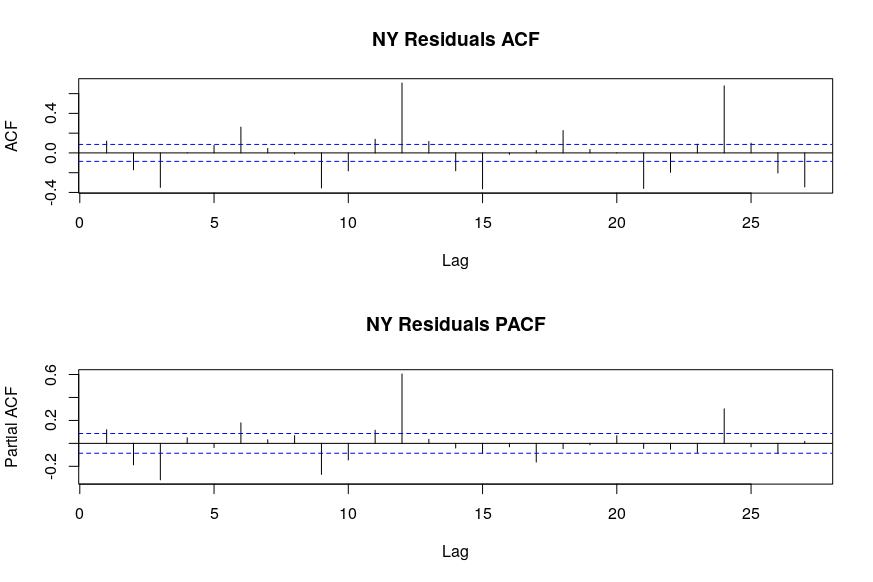
\includegraphics[width=380pt]{ny_residuals_acf}
	\caption{ARIMA Residual ACF and PACF for both states} 
\end{figure}


\noindent (f) The CUSUM for both ARIMA models are shown below. The CUSUM for our model for California indicates that while the model generally does a good job, it struggles at certain points in time, around t = 100, 200 and 400-470, which correspond to the years. 


\begin{figure}[H]
	
	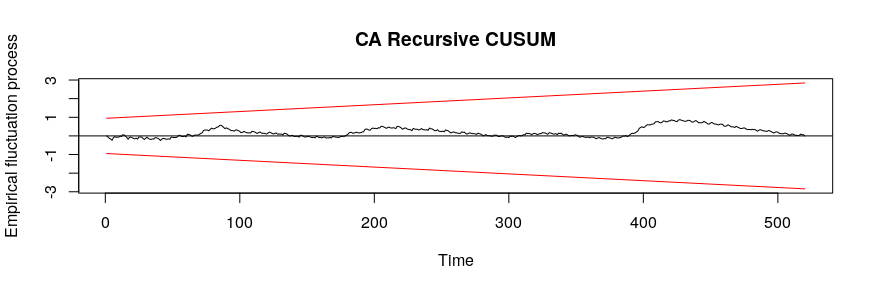
\includegraphics[width=\linewidth]{ca_cusum}
	\caption{California ARIMA Model CUSUM } 
\end{figure}


\begin{figure}[H]
	
	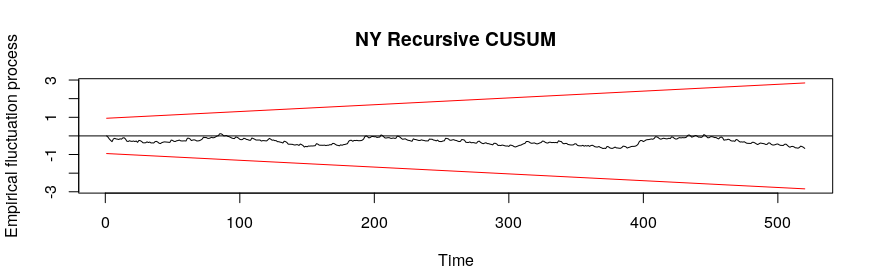
\includegraphics[width=\linewidth]{ny_cusum}
	\caption{New York ARIMA Model CUSUM } 
\end{figure}
\noindent The CUSUM for the New York model also fits well, but has trouble with the time periods t = 150, 300 and 350, which correspond to . \\


\noindent (g) The recursive residuals are show below:
\end{document}